
%*************************************************************************
% A Classic Thesis Style
% An Homage to The Elements of Typographic Style
%
% Copyright (C) 2017 André Miede and Ivo Pletikosić
%
% If you like the style then I would appreciate a postcard. My address
% can be found in the file ClassicThesis.pdf. A collection of the
% postcards I received so far is available online at
% http://postcards.miede.de
%
% License:
% This program is free software; you can redistribute it and/or modify
% it under the terms of the GNU General Public License as published by
% the Free Software Foundation; either version 2 of the License, or
% (at your option) any later version.
%
% This program is distributed in the hope that it will be useful,
% but WITHOUT ANY WARRANTY; without even the implied warranty of
% MERCHANTABILITY or FITNESS FOR A PARTICULAR PURPOSE.  See the
% GNU General Public License for more details.
%
% You should have received a copy of the GNU General Public License
% along with this program; see the file COPYING.  If not, write to
% the Free Software Foundation, Inc., 59 Temple Place - Suite 330,
% Boston, MA 02111-1307, USA.
%
% PLEASE SEE ALSO THE AUTHORS' NOTE REGARDING THIS LICENSE
% IN THE DOCUMENTATION (ClassicThesis.pdf --> Chapter 1 / Chapter01.tex)
%*************************************************************************
\RequirePackage{silence} % :-\
    \WarningFilter{scrreprt}{Usage of package `titlesec'}
    %\WarningFilter{scrreprt}{Activating an ugly workaround}
    \WarningFilter{titlesec}{Non standard sectioning command detected}
\documentclass[ openright,titlepage,numbers=noenddot,headinclude,%twoside, %1headlines,% letterpaper a4paper
                footinclude=true,cleardoublepage=empty,abstractoff, % <--- obsolete, remove (todo)
                BCOR=5mm,paper=a4,fontsize=11pt,%11pt,a4paper,%
                ngerman,american,%
                ]{scrreprt}
\usepackage{verbatim}
%*************************************************************************
% Note: Make all your adjustments in here
%*************************************************************************
% ****************************************************************************************************
% hdathesis-config.tex 
% Use it at the beginning of your thesis.tex, or as a LaTeX Preamble 
% in your thesis.{tex,lyx} with % ****************************************************************************************************
% hdathesis-config.tex 
% Use it at the beginning of your thesis.tex, or as a LaTeX Preamble 
% in your thesis.{tex,lyx} with % ****************************************************************************************************
% hdathesis-config.tex 
% Use it at the beginning of your thesis.tex, or as a LaTeX Preamble 
% in your thesis.{tex,lyx} with \input{hdathesis-config}
% ****************************************************************************************************

% ****************************************************************************************************
% 1. Personal data and user ad-hoc commands
% ****************************************************************************************************
\newcommand{\myTitle}{Möglichkeiten zur Erkennung von Thread Safety Problemen und deren Lösung\xspace}
%\newcommand{\mySubtitle}{An Homage to The Elements of Typographic Style\xspace}
\newcommand{\myDegree}{\xspace} 
%\newcommand{\myDegree}{Bachelor of Arts (B.A.)\xspace}
%\newcommand{\myDegree}{Master of Science (M.Sc.)\xspace}
%\newcommand{\myDegree}{Master of Arts (M.A.)\xspace}
\newcommand{\myName}{Tobias Renner\xspace}
\newcommand{\myId}{1113581\xspace}
\newcommand{\myProf}{Jens Karas\xspace}
\newcommand{\myOtherProf}{\xspace}
\newcommand{\myFaculty}{Fachbereich Informatik\xspace}
\newcommand{\myUni}{Hochschule Darmstadt\xspace}
\newcommand{\myLocation}{Darmstadt\xspace}
\newcommand{\myTime}{1. März 2023\xspace}
\newcommand{\myVersion}{version 4.4\xspace}

% ****************************************************************************************************
% 2. Is it a master thesis?
% ****************************************************************************************************
%\PassOptionsToPackage{master}{hdahesis} % uncomment if this is a master thesis 

% ****************************************************************************************************
% 3. Does the thesis have a lock flag?
% ****************************************************************************************************
%\PassOptionsToPackage{lockflag}{hdathesis} % uncomment if this thesis has a lock flag 

% ****************************************************************************************************
% 4. Loading some handy packages
% ****************************************************************************************************
% ****************************************************************************************************
% Packages with options that might require adjustments
% ****************************************************************************************************

%\PassOptionsToPackage{ngerman,american}{babel}   % change this to your language(s)
% Spanish languages need extra options in order to work with this template
%\PassOptionsToPackage{spanish,es-lcroman}{babel}
\usepackage{babel}
\usepackage{hyperref}

% ****************************************************************************************************

% ****************************************************************************************************
% 1. Personal data and user ad-hoc commands
% ****************************************************************************************************
\newcommand{\myTitle}{Möglichkeiten zur Erkennung von Thread Safety Problemen und deren Lösung\xspace}
%\newcommand{\mySubtitle}{An Homage to The Elements of Typographic Style\xspace}
\newcommand{\myDegree}{\xspace} 
%\newcommand{\myDegree}{Bachelor of Arts (B.A.)\xspace}
%\newcommand{\myDegree}{Master of Science (M.Sc.)\xspace}
%\newcommand{\myDegree}{Master of Arts (M.A.)\xspace}
\newcommand{\myName}{Tobias Renner\xspace}
\newcommand{\myId}{1113581\xspace}
\newcommand{\myProf}{Jens Karas\xspace}
\newcommand{\myOtherProf}{\xspace}
\newcommand{\myFaculty}{Fachbereich Informatik\xspace}
\newcommand{\myUni}{Hochschule Darmstadt\xspace}
\newcommand{\myLocation}{Darmstadt\xspace}
\newcommand{\myTime}{1. März 2023\xspace}
\newcommand{\myVersion}{version 4.4\xspace}

% ****************************************************************************************************
% 2. Is it a master thesis?
% ****************************************************************************************************
%\PassOptionsToPackage{master}{hdahesis} % uncomment if this is a master thesis 

% ****************************************************************************************************
% 3. Does the thesis have a lock flag?
% ****************************************************************************************************
%\PassOptionsToPackage{lockflag}{hdathesis} % uncomment if this thesis has a lock flag 

% ****************************************************************************************************
% 4. Loading some handy packages
% ****************************************************************************************************
% ****************************************************************************************************
% Packages with options that might require adjustments
% ****************************************************************************************************

%\PassOptionsToPackage{ngerman,american}{babel}   % change this to your language(s)
% Spanish languages need extra options in order to work with this template
%\PassOptionsToPackage{spanish,es-lcroman}{babel}
\usepackage{babel}
\usepackage{hyperref}

% ****************************************************************************************************

% ****************************************************************************************************
% 1. Personal data and user ad-hoc commands
% ****************************************************************************************************
\newcommand{\myTitle}{Möglichkeiten zur Erkennung von Thread Safety Problemen und deren Lösung\xspace}
%\newcommand{\mySubtitle}{An Homage to The Elements of Typographic Style\xspace}
\newcommand{\myDegree}{\xspace} 
%\newcommand{\myDegree}{Bachelor of Arts (B.A.)\xspace}
%\newcommand{\myDegree}{Master of Science (M.Sc.)\xspace}
%\newcommand{\myDegree}{Master of Arts (M.A.)\xspace}
\newcommand{\myName}{Tobias Renner\xspace}
\newcommand{\myId}{1113581\xspace}
\newcommand{\myProf}{Jens Karas\xspace}
\newcommand{\myOtherProf}{\xspace}
\newcommand{\myFaculty}{Fachbereich Informatik\xspace}
\newcommand{\myUni}{Hochschule Darmstadt\xspace}
\newcommand{\myLocation}{Darmstadt\xspace}
\newcommand{\myTime}{1. März 2023\xspace}
\newcommand{\myVersion}{version 4.4\xspace}

% ****************************************************************************************************
% 2. Is it a master thesis?
% ****************************************************************************************************
%\PassOptionsToPackage{master}{hdahesis} % uncomment if this is a master thesis 

% ****************************************************************************************************
% 3. Does the thesis have a lock flag?
% ****************************************************************************************************
%\PassOptionsToPackage{lockflag}{hdathesis} % uncomment if this thesis has a lock flag 

% ****************************************************************************************************
% 4. Loading some handy packages
% ****************************************************************************************************
% ****************************************************************************************************
% Packages with options that might require adjustments
% ****************************************************************************************************

%\PassOptionsToPackage{ngerman,american}{babel}   % change this to your language(s)
% Spanish languages need extra options in order to work with this template
%\PassOptionsToPackage{spanish,es-lcroman}{babel}
\usepackage{babel}
\usepackage{hyperref}

% ****************************************************************************************************
% classicthesis-config.tex
% formerly known as loadpackages.sty, classicthesis-ldpkg.sty, and classicthesis-preamble.sty
% Use it at the beginning of your ClassicThesis.tex, or as a LaTeX Preamble
% in your ClassicThesis.{tex,lyx} with % ****************************************************************************************************
% classicthesis-config.tex
% formerly known as loadpackages.sty, classicthesis-ldpkg.sty, and classicthesis-preamble.sty
% Use it at the beginning of your ClassicThesis.tex, or as a LaTeX Preamble
% in your ClassicThesis.{tex,lyx} with % ****************************************************************************************************
% classicthesis-config.tex
% formerly known as loadpackages.sty, classicthesis-ldpkg.sty, and classicthesis-preamble.sty
% Use it at the beginning of your ClassicThesis.tex, or as a LaTeX Preamble
% in your ClassicThesis.{tex,lyx} with \input{classicthesis-config}
% ****************************************************************************************************
% If you like the classicthesis, then I would appreciate a postcard.
% My address can be found in the file ClassicThesis.pdf. A collection
% of the postcards I received so far is available online at
% http://postcards.miede.de
% ****************************************************************************************************


% ****************************************************************************************************
% 0. Set the encoding of your files. UTF-8 is the only sensible encoding nowadays. If you can't read
% äöüßáéçèê∂åëæƒÏ€ then change the encoding setting in your editor, not the line below. If your editor
% does not support utf8 use another editor!
% ****************************************************************************************************
\PassOptionsToPackage{utf8}{inputenc}
  \usepackage{inputenc}

% ****************************************************************************************************
% 1. Configure classicthesis for your needs here, e.g., remove "drafting" below
% in order to deactivate the time-stamp on the pages
% (see ClassicThesis.pdf for more information):
% ****************************************************************************************************
\PassOptionsToPackage{
  drafting=false,   % print version information on the bottom of the pages
  tocaligned=false, % the left column of the toc will be aligned (no indentation)
  dottedtoc=true,   % page numbers in ToC flushed right
  parts=true,       % use part division
  eulerchapternumbers=true, % use AMS Euler for chapter font (otherwise Palatino)
  linedheaders=false,       % chaper headers will have line above and beneath
  floatperchapter=true,     % numbering per chapter for all floats (i.e., Figure 1.1)
  listings=true,    % load listings package and setup LoL
  subfig=true,      % setup for preloaded subfig package
  eulermath=false,  % use awesome Euler fonts for mathematical formulae (only with pdfLaTeX)
  beramono=true,    % toggle a nice monospaced font (w/ bold)
  minionpro=false   % setup for minion pro font; use minion pro small caps as well (only with pdfLaTeX)
}{classicthesis}


% ****************************************************************************************************
% 2. Personal data and user ad-hoc commands
% ****************************************************************************************************
%\newcommand{\myTitle}{A Classic Thesis Style\xspace}
%\newcommand{\mySubtitle}{An Homage to The Elements of Typographic Style\xspace}
%\newcommand{\myDegree}{Doktor-Ingenieur (Dr.-Ing.)\xspace}
%\newcommand{\myName}{André Miede\xspace}
%\newcommand{\myProf}{Put name here\xspace}
%\newcommand{\myOtherProf}{Put name here\xspace}
%\newcommand{\mySupervisor}{Put name here\xspace}
%\newcommand{\myFaculty}{Put data here\xspace}
%\newcommand{\myDepartment}{Put data here\xspace}
%\newcommand{\myUni}{Put data here\xspace}
%\newcommand{\myLocation}{Saarbrücken\xspace}
%\newcommand{\myTime}{October 2017\xspace}
%\newcommand{\myVersion}{version 4.4}

% ********************************************************************
% Setup, finetuning, and useful commands
% ********************************************************************
\newcounter{dummy} % necessary for correct hyperlinks (to index, bib, etc.)
\newlength{\abcd} % for ab..z string length calculation
\providecommand{\mLyX}{L\kern-.1667em\lower.25em\hbox{Y}\kern-.125emX\@}
\newcommand{\ie}{i.\,e.}
\newcommand{\Ie}{I.\,e.}
\newcommand{\eg}{e.\,g.}
\newcommand{\Eg}{E.\,g.}
% ****************************************************************************************************


% ****************************************************************************************************
% 3. Loading some handy packages
% ****************************************************************************************************
% ********************************************************************
% Packages with options that might require adjustments
% ********************************************************************
%\PassOptionsToPackage{ngerman,american}{babel}   % change this to your language(s), main language last
% Spanish languages need extra options in order to work with this template
%\PassOptionsToPackage{spanish,es-lcroman}{babel}
\usepackage{babel}

\usepackage{csquotes}

\PassOptionsToPackage{%
  %backend=biber,bibencoding=utf8, %instead of bibtex
  backend=bibtex8,bibencoding=ascii,%
  language=auto,%
  style=numeric-comp,%
  %style=alphabetic,%
  %style=authoryear-comp, % Author 1999, 2010
  %bibstyle=authoryear,dashed=false, % dashed: substitute rep. author with ---
  sorting=nyt, % name, year, title
  maxbibnames=10, % default: 3, et al.
  %backref=true,%
  natbib=true % natbib compatibility mode (\citep and \citet still work)
}{biblatex}
  \usepackage{biblatex}

\PassOptionsToPackage{fleqn}{amsmath}       % math environments and more by the AMS
  \usepackage{amsmath}

\PassOptionsToPackage{doublespacing}{hdathesis}  % options: abbrev exam big wiwi english master
  \usepackage{hdathesis}

% ********************************************************************
% General useful packages
% ********************************************************************
\PassOptionsToPackage{T1}{fontenc} % T2A for cyrillics
  \usepackage{fontenc}
\usepackage{textcomp} % fix warning with missing font shapes
\usepackage{scrhack} % fix warnings when using KOMA with listings package
\usepackage{xspace} % to get the spacing after macros right
\usepackage{mparhack} % get marginpar right
%\usepackage{fixltx2e} % fixes some LaTeX stuff --> since 2015 in the LaTeX kernel (see below)
% \usepackage[latest]{latexrelease} % emulate newer kernel version if older is detected
\PassOptionsToPackage{printonlyused,smaller}{acronym}
  \usepackage{acronym} % nice macros for handling all acronyms in the thesis
  %\renewcommand{\bflabel}[1]{{#1}\hfill} % fix the list of acronyms --> no longer working
  %\renewcommand*{\acsfont}[1]{\textsc{#1}}
  %\renewcommand*{\aclabelfont}[1]{\acsfont{#1}}
  %\def\bflabel#1{{#1\hfill}}
  \def\bflabel#1{{\acsfont{#1}\hfill}}
  \def\aclabelfont#1{\acsfont{#1}}
% ****************************************************************************************************
%\usepackage{pgfplots} % External TikZ/PGF support (thanks to Andreas Nautsch)
%\usetikzlibrary{external}
%\tikzexternalize[mode=list and make, prefix=ext-tikz/]
% ****************************************************************************************************


% ****************************************************************************************************
% 4. Setup floats: tables, (sub)figures, and captions
% ****************************************************************************************************
\usepackage{tabularx} % better tables
  \setlength{\extrarowheight}{3pt} % increase table row height
\newcommand{\tableheadline}[1]{\multicolumn{1}{c}{\spacedlowsmallcaps{#1}}}
\newcommand{\myfloatalign}{\centering} % to be used with each float for alignment
\usepackage{caption}
% Thanks to cgnieder and Claus Lahiri
% http://tex.stackexchange.com/questions/69349/spacedlowsmallcaps-in-caption-label
% [REMOVED DUE TO OTHER PROBLEMS, SEE ISSUE #82]
%\DeclareCaptionLabelFormat{smallcaps}{\bothIfFirst{#1}{~}\MakeTextLowercase{\textsc{#2}}}
%\captionsetup{font=small,labelformat=smallcaps} % format=hang,
\captionsetup{font=small} % format=hang,
\usepackage{subfig}
% ****************************************************************************************************


% ****************************************************************************************************
% 5. Setup code listings
% ****************************************************************************************************
\usepackage{listings}
%\lstset{emph={trueIndex,root},emphstyle=\color{BlueViolet}}%\underbar} % for special keywords
\lstset{language=[LaTeX]Tex,%C++,
  morekeywords={PassOptionsToPackage,selectlanguage},
  keywordstyle=\color{RoyalBlue},%\bfseries,
  basicstyle=\small\ttfamily,
  %identifierstyle=\color{NavyBlue},
  commentstyle=\color{Green}\ttfamily,
  stringstyle=\rmfamily,
  numbers=none,%left,%
  numberstyle=\scriptsize,%\tiny
  stepnumber=5,
  numbersep=8pt,
  showstringspaces=false,
  breaklines=true,
  %frameround=ftff,
  %frame=single,
  belowcaptionskip=.75\baselineskip
  %frame=L
}
% ****************************************************************************************************


% ****************************************************************************************************
% 6. PDFLaTeX, hyperreferences, and citation backreferences
% ****************************************************************************************************
% ********************************************************************
% Using PDFLaTeX
% ********************************************************************
\PassOptionsToPackage{hyperfootnotes=false,pdfpagelabels}{hyperref}
  \usepackage{hyperref}  % backref linktocpage pagebackref
%\ifpdf
%\pdfcompresslevel=9
%\pdfadjustspacing=1
%\fi
%\PassOptionsToPackage{pdftex}{graphicx} %%%IVO: driver will be chosen automatically
  \usepackage{graphicx}


% ********************************************************************
% Hyperreferences
% ********************************************************************
\hypersetup{%
  %draft, % hyperref's draft mode, for printing see below
  colorlinks=true, linktocpage=true, pdfstartpage=3, pdfstartview=FitV,%
  % uncomment the following line if you want to have black links (e.g., for printing)
  %colorlinks=false, linktocpage=false, pdfstartpage=3, pdfstartview=FitV, pdfborder={0 0 0},%
  breaklinks=true, pdfpagemode=UseNone, pageanchor=true, pdfpagemode=UseOutlines,%
  plainpages=false, bookmarksnumbered, bookmarksopen=true, bookmarksopenlevel=1,%
  hypertexnames=true, pdfhighlight=/O,%nesting=true,%frenchlinks,%
  urlcolor=webbrown, linkcolor=RoyalBlue, citecolor=webgreen, %pagecolor=RoyalBlue,%
  %urlcolor=Black, linkcolor=Black, citecolor=Black, %pagecolor=Black,%
  pdftitle={\myTitle},%
  pdfauthor={\textcopyright\ \myName, \myUni, \myFaculty},%
  pdfsubject={},%
  pdfkeywords={},%
  pdfcreator={pdfLaTeX},%
  pdfproducer={LaTeX with hyperref and classicthesis}%
}

% ********************************************************************
% Setup autoreferences
% ********************************************************************
% There are some issues regarding autorefnames
% http://www.ureader.de/msg/136221647.aspx
% http://www.tex.ac.uk/cgi-bin/texfaq2html?label=latexwords
% you have to redefine the makros for the
% language you use, e.g., american, ngerman
% (as chosen when loading babel/AtBeginDocument)
% ********************************************************************
\makeatletter
\@ifpackageloaded{babel}%
  {%
    \addto\extrasamerican{%
      \renewcommand*{\figureautorefname}{Figure}%
      \renewcommand*{\tableautorefname}{Table}%
      \renewcommand*{\partautorefname}{Part}%
      \renewcommand*{\chapterautorefname}{Chapter}%
      \renewcommand*{\sectionautorefname}{Section}%
      \renewcommand*{\subsectionautorefname}{Section}%
      \renewcommand*{\subsubsectionautorefname}{Section}%
    }%
    \addto\extrasngerman{%
      \renewcommand*{\paragraphautorefname}{Absatz}%
      \renewcommand*{\subparagraphautorefname}{Unterabsatz}%
      \renewcommand*{\footnoteautorefname}{Fu\"snote}%
      \renewcommand*{\FancyVerbLineautorefname}{Zeile}%
      \renewcommand*{\theoremautorefname}{Theorem}%
      \renewcommand*{\appendixautorefname}{Anhang}%
      \renewcommand*{\equationautorefname}{Gleichung}%
      \renewcommand*{\itemautorefname}{Punkt}%
    }%
      % Fix to getting autorefs for subfigures right (thanks to Belinda Vogt for changing the definition)
      \providecommand{\subfigureautorefname}{\figureautorefname}%
    }{\relax}
\makeatother


% ****************************************************************************************************
% 7. Last calls before the bar closes
% ****************************************************************************************************
% ********************************************************************
% Development Stuff
% ********************************************************************
\listfiles
%\PassOptionsToPackage{l2tabu,orthodox,abort}{nag}
%  \usepackage{nag}
%\PassOptionsToPackage{warning, all}{onlyamsmath}
%  \usepackage{onlyamsmath}

% ********************************************************************
% Last, but not least...
% ********************************************************************
\usepackage{classicthesis}
% ****************************************************************************************************


% ****************************************************************************************************
% 8. Further adjustments (experimental)
% ****************************************************************************************************
% ********************************************************************
% Changing the text area
% ********************************************************************
%\areaset[current]{312pt}{761pt} % 686 (factor 2.2) + 33 head + 42 head \the\footskip
%\setlength{\marginparwidth}{7em}%
%\setlength{\marginparsep}{2em}%

% ********************************************************************
% Using different fonts
% ********************************************************************
%\usepackage[oldstylenums]{kpfonts} % oldstyle notextcomp
%\usepackage[osf]{libertine}
%\usepackage[light,condensed,math]{iwona}
%\renewcommand{\sfdefault}{iwona}
%\usepackage{lmodern} % <-- no osf support :-(
%\usepackage{cfr-lm} %
%\usepackage[urw-garamond]{mathdesign} <-- no osf support :-(
%\usepackage[default,osfigures]{opensans} % scale=0.95
%\usepackage[sfdefault]{FiraSans}
% ********************************************************************
% \usepackage[largesc,osf]{newpxtext}
% Used to fix these:
% https://bitbucket.org/amiede/classicthesis/issues/139/italics-in-pallatino-capitals-chapter
% https://bitbucket.org/amiede/classicthesis/issues/45/problema-testatine-su-classicthesis-style
% ********************************************************************
%\linespread{1.05} % a bit more for Palatino
% ****************************************************************************************************

% ****************************************************************************************************
% If you like the classicthesis, then I would appreciate a postcard.
% My address can be found in the file ClassicThesis.pdf. A collection
% of the postcards I received so far is available online at
% http://postcards.miede.de
% ****************************************************************************************************


% ****************************************************************************************************
% 0. Set the encoding of your files. UTF-8 is the only sensible encoding nowadays. If you can't read
% äöüßáéçèê∂åëæƒÏ€ then change the encoding setting in your editor, not the line below. If your editor
% does not support utf8 use another editor!
% ****************************************************************************************************
\PassOptionsToPackage{utf8}{inputenc}
  \usepackage{inputenc}

% ****************************************************************************************************
% 1. Configure classicthesis for your needs here, e.g., remove "drafting" below
% in order to deactivate the time-stamp on the pages
% (see ClassicThesis.pdf for more information):
% ****************************************************************************************************
\PassOptionsToPackage{
  drafting=false,   % print version information on the bottom of the pages
  tocaligned=false, % the left column of the toc will be aligned (no indentation)
  dottedtoc=true,   % page numbers in ToC flushed right
  parts=true,       % use part division
  eulerchapternumbers=true, % use AMS Euler for chapter font (otherwise Palatino)
  linedheaders=false,       % chaper headers will have line above and beneath
  floatperchapter=true,     % numbering per chapter for all floats (i.e., Figure 1.1)
  listings=true,    % load listings package and setup LoL
  subfig=true,      % setup for preloaded subfig package
  eulermath=false,  % use awesome Euler fonts for mathematical formulae (only with pdfLaTeX)
  beramono=true,    % toggle a nice monospaced font (w/ bold)
  minionpro=false   % setup for minion pro font; use minion pro small caps as well (only with pdfLaTeX)
}{classicthesis}


% ****************************************************************************************************
% 2. Personal data and user ad-hoc commands
% ****************************************************************************************************
%\newcommand{\myTitle}{A Classic Thesis Style\xspace}
%\newcommand{\mySubtitle}{An Homage to The Elements of Typographic Style\xspace}
%\newcommand{\myDegree}{Doktor-Ingenieur (Dr.-Ing.)\xspace}
%\newcommand{\myName}{André Miede\xspace}
%\newcommand{\myProf}{Put name here\xspace}
%\newcommand{\myOtherProf}{Put name here\xspace}
%\newcommand{\mySupervisor}{Put name here\xspace}
%\newcommand{\myFaculty}{Put data here\xspace}
%\newcommand{\myDepartment}{Put data here\xspace}
%\newcommand{\myUni}{Put data here\xspace}
%\newcommand{\myLocation}{Saarbrücken\xspace}
%\newcommand{\myTime}{October 2017\xspace}
%\newcommand{\myVersion}{version 4.4}

% ********************************************************************
% Setup, finetuning, and useful commands
% ********************************************************************
\newcounter{dummy} % necessary for correct hyperlinks (to index, bib, etc.)
\newlength{\abcd} % for ab..z string length calculation
\providecommand{\mLyX}{L\kern-.1667em\lower.25em\hbox{Y}\kern-.125emX\@}
\newcommand{\ie}{i.\,e.}
\newcommand{\Ie}{I.\,e.}
\newcommand{\eg}{e.\,g.}
\newcommand{\Eg}{E.\,g.}
% ****************************************************************************************************


% ****************************************************************************************************
% 3. Loading some handy packages
% ****************************************************************************************************
% ********************************************************************
% Packages with options that might require adjustments
% ********************************************************************
%\PassOptionsToPackage{ngerman,american}{babel}   % change this to your language(s), main language last
% Spanish languages need extra options in order to work with this template
%\PassOptionsToPackage{spanish,es-lcroman}{babel}
\usepackage{babel}

\usepackage{csquotes}

\PassOptionsToPackage{%
  %backend=biber,bibencoding=utf8, %instead of bibtex
  backend=bibtex8,bibencoding=ascii,%
  language=auto,%
  style=numeric-comp,%
  %style=alphabetic,%
  %style=authoryear-comp, % Author 1999, 2010
  %bibstyle=authoryear,dashed=false, % dashed: substitute rep. author with ---
  sorting=nyt, % name, year, title
  maxbibnames=10, % default: 3, et al.
  %backref=true,%
  natbib=true % natbib compatibility mode (\citep and \citet still work)
}{biblatex}
  \usepackage{biblatex}

\PassOptionsToPackage{fleqn}{amsmath}       % math environments and more by the AMS
  \usepackage{amsmath}

\PassOptionsToPackage{doublespacing}{hdathesis}  % options: abbrev exam big wiwi english master
  \usepackage{hdathesis}

% ********************************************************************
% General useful packages
% ********************************************************************
\PassOptionsToPackage{T1}{fontenc} % T2A for cyrillics
  \usepackage{fontenc}
\usepackage{textcomp} % fix warning with missing font shapes
\usepackage{scrhack} % fix warnings when using KOMA with listings package
\usepackage{xspace} % to get the spacing after macros right
\usepackage{mparhack} % get marginpar right
%\usepackage{fixltx2e} % fixes some LaTeX stuff --> since 2015 in the LaTeX kernel (see below)
% \usepackage[latest]{latexrelease} % emulate newer kernel version if older is detected
\PassOptionsToPackage{printonlyused,smaller}{acronym}
  \usepackage{acronym} % nice macros for handling all acronyms in the thesis
  %\renewcommand{\bflabel}[1]{{#1}\hfill} % fix the list of acronyms --> no longer working
  %\renewcommand*{\acsfont}[1]{\textsc{#1}}
  %\renewcommand*{\aclabelfont}[1]{\acsfont{#1}}
  %\def\bflabel#1{{#1\hfill}}
  \def\bflabel#1{{\acsfont{#1}\hfill}}
  \def\aclabelfont#1{\acsfont{#1}}
% ****************************************************************************************************
%\usepackage{pgfplots} % External TikZ/PGF support (thanks to Andreas Nautsch)
%\usetikzlibrary{external}
%\tikzexternalize[mode=list and make, prefix=ext-tikz/]
% ****************************************************************************************************


% ****************************************************************************************************
% 4. Setup floats: tables, (sub)figures, and captions
% ****************************************************************************************************
\usepackage{tabularx} % better tables
  \setlength{\extrarowheight}{3pt} % increase table row height
\newcommand{\tableheadline}[1]{\multicolumn{1}{c}{\spacedlowsmallcaps{#1}}}
\newcommand{\myfloatalign}{\centering} % to be used with each float for alignment
\usepackage{caption}
% Thanks to cgnieder and Claus Lahiri
% http://tex.stackexchange.com/questions/69349/spacedlowsmallcaps-in-caption-label
% [REMOVED DUE TO OTHER PROBLEMS, SEE ISSUE #82]
%\DeclareCaptionLabelFormat{smallcaps}{\bothIfFirst{#1}{~}\MakeTextLowercase{\textsc{#2}}}
%\captionsetup{font=small,labelformat=smallcaps} % format=hang,
\captionsetup{font=small} % format=hang,
\usepackage{subfig}
% ****************************************************************************************************


% ****************************************************************************************************
% 5. Setup code listings
% ****************************************************************************************************
\usepackage{listings}
%\lstset{emph={trueIndex,root},emphstyle=\color{BlueViolet}}%\underbar} % for special keywords
\lstset{language=[LaTeX]Tex,%C++,
  morekeywords={PassOptionsToPackage,selectlanguage},
  keywordstyle=\color{RoyalBlue},%\bfseries,
  basicstyle=\small\ttfamily,
  %identifierstyle=\color{NavyBlue},
  commentstyle=\color{Green}\ttfamily,
  stringstyle=\rmfamily,
  numbers=none,%left,%
  numberstyle=\scriptsize,%\tiny
  stepnumber=5,
  numbersep=8pt,
  showstringspaces=false,
  breaklines=true,
  %frameround=ftff,
  %frame=single,
  belowcaptionskip=.75\baselineskip
  %frame=L
}
% ****************************************************************************************************


% ****************************************************************************************************
% 6. PDFLaTeX, hyperreferences, and citation backreferences
% ****************************************************************************************************
% ********************************************************************
% Using PDFLaTeX
% ********************************************************************
\PassOptionsToPackage{hyperfootnotes=false,pdfpagelabels}{hyperref}
  \usepackage{hyperref}  % backref linktocpage pagebackref
%\ifpdf
%\pdfcompresslevel=9
%\pdfadjustspacing=1
%\fi
%\PassOptionsToPackage{pdftex}{graphicx} %%%IVO: driver will be chosen automatically
  \usepackage{graphicx}


% ********************************************************************
% Hyperreferences
% ********************************************************************
\hypersetup{%
  %draft, % hyperref's draft mode, for printing see below
  colorlinks=true, linktocpage=true, pdfstartpage=3, pdfstartview=FitV,%
  % uncomment the following line if you want to have black links (e.g., for printing)
  %colorlinks=false, linktocpage=false, pdfstartpage=3, pdfstartview=FitV, pdfborder={0 0 0},%
  breaklinks=true, pdfpagemode=UseNone, pageanchor=true, pdfpagemode=UseOutlines,%
  plainpages=false, bookmarksnumbered, bookmarksopen=true, bookmarksopenlevel=1,%
  hypertexnames=true, pdfhighlight=/O,%nesting=true,%frenchlinks,%
  urlcolor=webbrown, linkcolor=RoyalBlue, citecolor=webgreen, %pagecolor=RoyalBlue,%
  %urlcolor=Black, linkcolor=Black, citecolor=Black, %pagecolor=Black,%
  pdftitle={\myTitle},%
  pdfauthor={\textcopyright\ \myName, \myUni, \myFaculty},%
  pdfsubject={},%
  pdfkeywords={},%
  pdfcreator={pdfLaTeX},%
  pdfproducer={LaTeX with hyperref and classicthesis}%
}

% ********************************************************************
% Setup autoreferences
% ********************************************************************
% There are some issues regarding autorefnames
% http://www.ureader.de/msg/136221647.aspx
% http://www.tex.ac.uk/cgi-bin/texfaq2html?label=latexwords
% you have to redefine the makros for the
% language you use, e.g., american, ngerman
% (as chosen when loading babel/AtBeginDocument)
% ********************************************************************
\makeatletter
\@ifpackageloaded{babel}%
  {%
    \addto\extrasamerican{%
      \renewcommand*{\figureautorefname}{Figure}%
      \renewcommand*{\tableautorefname}{Table}%
      \renewcommand*{\partautorefname}{Part}%
      \renewcommand*{\chapterautorefname}{Chapter}%
      \renewcommand*{\sectionautorefname}{Section}%
      \renewcommand*{\subsectionautorefname}{Section}%
      \renewcommand*{\subsubsectionautorefname}{Section}%
    }%
    \addto\extrasngerman{%
      \renewcommand*{\paragraphautorefname}{Absatz}%
      \renewcommand*{\subparagraphautorefname}{Unterabsatz}%
      \renewcommand*{\footnoteautorefname}{Fu\"snote}%
      \renewcommand*{\FancyVerbLineautorefname}{Zeile}%
      \renewcommand*{\theoremautorefname}{Theorem}%
      \renewcommand*{\appendixautorefname}{Anhang}%
      \renewcommand*{\equationautorefname}{Gleichung}%
      \renewcommand*{\itemautorefname}{Punkt}%
    }%
      % Fix to getting autorefs for subfigures right (thanks to Belinda Vogt for changing the definition)
      \providecommand{\subfigureautorefname}{\figureautorefname}%
    }{\relax}
\makeatother


% ****************************************************************************************************
% 7. Last calls before the bar closes
% ****************************************************************************************************
% ********************************************************************
% Development Stuff
% ********************************************************************
\listfiles
%\PassOptionsToPackage{l2tabu,orthodox,abort}{nag}
%  \usepackage{nag}
%\PassOptionsToPackage{warning, all}{onlyamsmath}
%  \usepackage{onlyamsmath}

% ********************************************************************
% Last, but not least...
% ********************************************************************
\usepackage{classicthesis}
% ****************************************************************************************************


% ****************************************************************************************************
% 8. Further adjustments (experimental)
% ****************************************************************************************************
% ********************************************************************
% Changing the text area
% ********************************************************************
%\areaset[current]{312pt}{761pt} % 686 (factor 2.2) + 33 head + 42 head \the\footskip
%\setlength{\marginparwidth}{7em}%
%\setlength{\marginparsep}{2em}%

% ********************************************************************
% Using different fonts
% ********************************************************************
%\usepackage[oldstylenums]{kpfonts} % oldstyle notextcomp
%\usepackage[osf]{libertine}
%\usepackage[light,condensed,math]{iwona}
%\renewcommand{\sfdefault}{iwona}
%\usepackage{lmodern} % <-- no osf support :-(
%\usepackage{cfr-lm} %
%\usepackage[urw-garamond]{mathdesign} <-- no osf support :-(
%\usepackage[default,osfigures]{opensans} % scale=0.95
%\usepackage[sfdefault]{FiraSans}
% ********************************************************************
% \usepackage[largesc,osf]{newpxtext}
% Used to fix these:
% https://bitbucket.org/amiede/classicthesis/issues/139/italics-in-pallatino-capitals-chapter
% https://bitbucket.org/amiede/classicthesis/issues/45/problema-testatine-su-classicthesis-style
% ********************************************************************
%\linespread{1.05} % a bit more for Palatino
% ****************************************************************************************************

% ****************************************************************************************************
% If you like the classicthesis, then I would appreciate a postcard.
% My address can be found in the file ClassicThesis.pdf. A collection
% of the postcards I received so far is available online at
% http://postcards.miede.de
% ****************************************************************************************************


% ****************************************************************************************************
% 0. Set the encoding of your files. UTF-8 is the only sensible encoding nowadays. If you can't read
% äöüßáéçèê∂åëæƒÏ€ then change the encoding setting in your editor, not the line below. If your editor
% does not support utf8 use another editor!
% ****************************************************************************************************
\PassOptionsToPackage{utf8}{inputenc}
  \usepackage{inputenc}

% ****************************************************************************************************
% 1. Configure classicthesis for your needs here, e.g., remove "drafting" below
% in order to deactivate the time-stamp on the pages
% (see ClassicThesis.pdf for more information):
% ****************************************************************************************************
\PassOptionsToPackage{
  drafting=false,   % print version information on the bottom of the pages
  tocaligned=false, % the left column of the toc will be aligned (no indentation)
  dottedtoc=true,   % page numbers in ToC flushed right
  parts=true,       % use part division
  eulerchapternumbers=true, % use AMS Euler for chapter font (otherwise Palatino)
  linedheaders=false,       % chaper headers will have line above and beneath
  floatperchapter=true,     % numbering per chapter for all floats (i.e., Figure 1.1)
  listings=true,    % load listings package and setup LoL
  subfig=true,      % setup for preloaded subfig package
  eulermath=false,  % use awesome Euler fonts for mathematical formulae (only with pdfLaTeX)
  beramono=true,    % toggle a nice monospaced font (w/ bold)
  minionpro=false   % setup for minion pro font; use minion pro small caps as well (only with pdfLaTeX)
}{classicthesis}


% ****************************************************************************************************
% 2. Personal data and user ad-hoc commands
% ****************************************************************************************************
%\newcommand{\myTitle}{A Classic Thesis Style\xspace}
%\newcommand{\mySubtitle}{An Homage to The Elements of Typographic Style\xspace}
%\newcommand{\myDegree}{Doktor-Ingenieur (Dr.-Ing.)\xspace}
%\newcommand{\myName}{André Miede\xspace}
%\newcommand{\myProf}{Put name here\xspace}
%\newcommand{\myOtherProf}{Put name here\xspace}
%\newcommand{\mySupervisor}{Put name here\xspace}
%\newcommand{\myFaculty}{Put data here\xspace}
%\newcommand{\myDepartment}{Put data here\xspace}
%\newcommand{\myUni}{Put data here\xspace}
%\newcommand{\myLocation}{Saarbrücken\xspace}
%\newcommand{\myTime}{October 2017\xspace}
%\newcommand{\myVersion}{version 4.4}

% ********************************************************************
% Setup, finetuning, and useful commands
% ********************************************************************
\newcounter{dummy} % necessary for correct hyperlinks (to index, bib, etc.)
\newlength{\abcd} % for ab..z string length calculation
\providecommand{\mLyX}{L\kern-.1667em\lower.25em\hbox{Y}\kern-.125emX\@}
\newcommand{\ie}{i.\,e.}
\newcommand{\Ie}{I.\,e.}
\newcommand{\eg}{e.\,g.}
\newcommand{\Eg}{E.\,g.}
% ****************************************************************************************************


% ****************************************************************************************************
% 3. Loading some handy packages
% ****************************************************************************************************
% ********************************************************************
% Packages with options that might require adjustments
% ********************************************************************
%\PassOptionsToPackage{ngerman,american}{babel}   % change this to your language(s), main language last
% Spanish languages need extra options in order to work with this template
%\PassOptionsToPackage{spanish,es-lcroman}{babel}
\usepackage{babel}

\usepackage{csquotes}

\PassOptionsToPackage{%
  %backend=biber,bibencoding=utf8, %instead of bibtex
  backend=bibtex8,bibencoding=ascii,%
  language=auto,%
  style=numeric-comp,%
  %style=alphabetic,%
  %style=authoryear-comp, % Author 1999, 2010
  %bibstyle=authoryear,dashed=false, % dashed: substitute rep. author with ---
  sorting=nyt, % name, year, title
  maxbibnames=10, % default: 3, et al.
  %backref=true,%
  natbib=true % natbib compatibility mode (\citep and \citet still work)
}{biblatex}
  \usepackage{biblatex}

\PassOptionsToPackage{fleqn}{amsmath}       % math environments and more by the AMS
  \usepackage{amsmath}

\PassOptionsToPackage{doublespacing}{hdathesis}  % options: abbrev exam big wiwi english master
  \usepackage{hdathesis}

% ********************************************************************
% General useful packages
% ********************************************************************
\PassOptionsToPackage{T1}{fontenc} % T2A for cyrillics
  \usepackage{fontenc}
\usepackage{textcomp} % fix warning with missing font shapes
\usepackage{scrhack} % fix warnings when using KOMA with listings package
\usepackage{xspace} % to get the spacing after macros right
\usepackage{mparhack} % get marginpar right
%\usepackage{fixltx2e} % fixes some LaTeX stuff --> since 2015 in the LaTeX kernel (see below)
% \usepackage[latest]{latexrelease} % emulate newer kernel version if older is detected
\PassOptionsToPackage{printonlyused,smaller}{acronym}
  \usepackage{acronym} % nice macros for handling all acronyms in the thesis
  %\renewcommand{\bflabel}[1]{{#1}\hfill} % fix the list of acronyms --> no longer working
  %\renewcommand*{\acsfont}[1]{\textsc{#1}}
  %\renewcommand*{\aclabelfont}[1]{\acsfont{#1}}
  %\def\bflabel#1{{#1\hfill}}
  \def\bflabel#1{{\acsfont{#1}\hfill}}
  \def\aclabelfont#1{\acsfont{#1}}
% ****************************************************************************************************
%\usepackage{pgfplots} % External TikZ/PGF support (thanks to Andreas Nautsch)
%\usetikzlibrary{external}
%\tikzexternalize[mode=list and make, prefix=ext-tikz/]
% ****************************************************************************************************


% ****************************************************************************************************
% 4. Setup floats: tables, (sub)figures, and captions
% ****************************************************************************************************
\usepackage{tabularx} % better tables
  \setlength{\extrarowheight}{3pt} % increase table row height
\newcommand{\tableheadline}[1]{\multicolumn{1}{c}{\spacedlowsmallcaps{#1}}}
\newcommand{\myfloatalign}{\centering} % to be used with each float for alignment
\usepackage{caption}
% Thanks to cgnieder and Claus Lahiri
% http://tex.stackexchange.com/questions/69349/spacedlowsmallcaps-in-caption-label
% [REMOVED DUE TO OTHER PROBLEMS, SEE ISSUE #82]
%\DeclareCaptionLabelFormat{smallcaps}{\bothIfFirst{#1}{~}\MakeTextLowercase{\textsc{#2}}}
%\captionsetup{font=small,labelformat=smallcaps} % format=hang,
\captionsetup{font=small} % format=hang,
\usepackage{subfig}
% ****************************************************************************************************


% ****************************************************************************************************
% 5. Setup code listings
% ****************************************************************************************************
\usepackage{listings}
%\lstset{emph={trueIndex,root},emphstyle=\color{BlueViolet}}%\underbar} % for special keywords
\lstset{language=[LaTeX]Tex,%C++,
  morekeywords={PassOptionsToPackage,selectlanguage},
  keywordstyle=\color{RoyalBlue},%\bfseries,
  basicstyle=\small\ttfamily,
  %identifierstyle=\color{NavyBlue},
  commentstyle=\color{Green}\ttfamily,
  stringstyle=\rmfamily,
  numbers=none,%left,%
  numberstyle=\scriptsize,%\tiny
  stepnumber=5,
  numbersep=8pt,
  showstringspaces=false,
  breaklines=true,
  %frameround=ftff,
  %frame=single,
  belowcaptionskip=.75\baselineskip
  %frame=L
}
% ****************************************************************************************************


% ****************************************************************************************************
% 6. PDFLaTeX, hyperreferences, and citation backreferences
% ****************************************************************************************************
% ********************************************************************
% Using PDFLaTeX
% ********************************************************************
\PassOptionsToPackage{hyperfootnotes=false,pdfpagelabels}{hyperref}
  \usepackage{hyperref}  % backref linktocpage pagebackref
%\ifpdf
%\pdfcompresslevel=9
%\pdfadjustspacing=1
%\fi
%\PassOptionsToPackage{pdftex}{graphicx} %%%IVO: driver will be chosen automatically
  \usepackage{graphicx}


% ********************************************************************
% Hyperreferences
% ********************************************************************
\hypersetup{%
  %draft, % hyperref's draft mode, for printing see below
  colorlinks=true, linktocpage=true, pdfstartpage=3, pdfstartview=FitV,%
  % uncomment the following line if you want to have black links (e.g., for printing)
  %colorlinks=false, linktocpage=false, pdfstartpage=3, pdfstartview=FitV, pdfborder={0 0 0},%
  breaklinks=true, pdfpagemode=UseNone, pageanchor=true, pdfpagemode=UseOutlines,%
  plainpages=false, bookmarksnumbered, bookmarksopen=true, bookmarksopenlevel=1,%
  hypertexnames=true, pdfhighlight=/O,%nesting=true,%frenchlinks,%
  urlcolor=webbrown, linkcolor=RoyalBlue, citecolor=webgreen, %pagecolor=RoyalBlue,%
  %urlcolor=Black, linkcolor=Black, citecolor=Black, %pagecolor=Black,%
  pdftitle={\myTitle},%
  pdfauthor={\textcopyright\ \myName, \myUni, \myFaculty},%
  pdfsubject={},%
  pdfkeywords={},%
  pdfcreator={pdfLaTeX},%
  pdfproducer={LaTeX with hyperref and classicthesis}%
}

% ********************************************************************
% Setup autoreferences
% ********************************************************************
% There are some issues regarding autorefnames
% http://www.ureader.de/msg/136221647.aspx
% http://www.tex.ac.uk/cgi-bin/texfaq2html?label=latexwords
% you have to redefine the makros for the
% language you use, e.g., american, ngerman
% (as chosen when loading babel/AtBeginDocument)
% ********************************************************************
\makeatletter
\@ifpackageloaded{babel}%
  {%
    \addto\extrasamerican{%
      \renewcommand*{\figureautorefname}{Figure}%
      \renewcommand*{\tableautorefname}{Table}%
      \renewcommand*{\partautorefname}{Part}%
      \renewcommand*{\chapterautorefname}{Chapter}%
      \renewcommand*{\sectionautorefname}{Section}%
      \renewcommand*{\subsectionautorefname}{Section}%
      \renewcommand*{\subsubsectionautorefname}{Section}%
    }%
    \addto\extrasngerman{%
      \renewcommand*{\paragraphautorefname}{Absatz}%
      \renewcommand*{\subparagraphautorefname}{Unterabsatz}%
      \renewcommand*{\footnoteautorefname}{Fu\"snote}%
      \renewcommand*{\FancyVerbLineautorefname}{Zeile}%
      \renewcommand*{\theoremautorefname}{Theorem}%
      \renewcommand*{\appendixautorefname}{Anhang}%
      \renewcommand*{\equationautorefname}{Gleichung}%
      \renewcommand*{\itemautorefname}{Punkt}%
    }%
      % Fix to getting autorefs for subfigures right (thanks to Belinda Vogt for changing the definition)
      \providecommand{\subfigureautorefname}{\figureautorefname}%
    }{\relax}
\makeatother


% ****************************************************************************************************
% 7. Last calls before the bar closes
% ****************************************************************************************************
% ********************************************************************
% Development Stuff
% ********************************************************************
\listfiles
%\PassOptionsToPackage{l2tabu,orthodox,abort}{nag}
%  \usepackage{nag}
%\PassOptionsToPackage{warning, all}{onlyamsmath}
%  \usepackage{onlyamsmath}

% ********************************************************************
% Last, but not least...
% ********************************************************************
\usepackage{classicthesis}
% ****************************************************************************************************


% ****************************************************************************************************
% 8. Further adjustments (experimental)
% ****************************************************************************************************
% ********************************************************************
% Changing the text area
% ********************************************************************
%\areaset[current]{312pt}{761pt} % 686 (factor 2.2) + 33 head + 42 head \the\footskip
%\setlength{\marginparwidth}{7em}%
%\setlength{\marginparsep}{2em}%

% ********************************************************************
% Using different fonts
% ********************************************************************
%\usepackage[oldstylenums]{kpfonts} % oldstyle notextcomp
%\usepackage[osf]{libertine}
%\usepackage[light,condensed,math]{iwona}
%\renewcommand{\sfdefault}{iwona}
%\usepackage{lmodern} % <-- no osf support :-(
%\usepackage{cfr-lm} %
%\usepackage[urw-garamond]{mathdesign} <-- no osf support :-(
%\usepackage[default,osfigures]{opensans} % scale=0.95
%\usepackage[sfdefault]{FiraSans}
% ********************************************************************
% \usepackage[largesc,osf]{newpxtext}
% Used to fix these:
% https://bitbucket.org/amiede/classicthesis/issues/139/italics-in-pallatino-capitals-chapter
% https://bitbucket.org/amiede/classicthesis/issues/45/problema-testatine-su-classicthesis-style
% ********************************************************************
%\linespread{1.05} % a bit more for Palatino
% ****************************************************************************************************


%*************************************************************************
% Bibliographies
%*************************************************************************
\addbibresource{bibliography.bib}

%*************************************************************************
% Hyphenation
%*************************************************************************
%\hyphenation{put special hyphenation here}

%*************************************************************************
% GO!GO!GO! MOVE IT!
%*************************************************************************
\begin{document}
\frenchspacing
\raggedbottom
\selectlanguage{ngerman} % ngerman, american
%\renewcommand*{\bibname}{new name}
%\setbibpreamble{}
\pagenumbering{roman}
\pagestyle{plain}
%*************************************************************************
% Frontmatter
%*************************************************************************
%*******************************************************
% Titlepage
%*******************************************************
%%%
%%% title page (german)
%%%
\thispagestyle{empty}
\pdfbookmark[0]{Titelblatt}{title}
\begin{titlepage}

  % If printed on two sides, center the title page
  \condTWOSIDE{\changetext{}{19mm}{}{19mm}{}}

  \vspace{1cm}
  \begin{center}
    
\includegraphics[width=7.7cm]{gfx/logo_h-da_rot} \\ 
  \end{center}

  \begin{center}
    \vspace{0.1cm}
    \huge \textbf{\myUni}\\
    \vspace{0.4cm}
    \LARGE -- \myFaculty --
  \end{center}

  \vfill
  \vfill

  \begin{center}
    \LARGE \textbf{\myTitle}
  \end{center} 

  \vfill
  \vfill

  \begin{center}
    \Large Wissenschaftliche Arbeit zu einem aktuellen Thema der Informatik\\
    \vspace{0.3cm}
    \Large \myDegree
  \end{center}

  \vfill

  \begin{center}
    \Large vorgelegt von\\
    \vspace{0.3cm}
    \Large \textbf{\myName}\\
    \vspace{0.3cm}
    \normalsize Matrikelnummer: \myId
  \end{center}

  \vfill
  \vfill

  \begin{center}
    \begin{tabular}{lll}
      Referent    & : & \myProf 
    \end{tabular}
  \end{center} 

  % If printed on two sides, center the title page
  \condTWOSIDE{\changetext{}{-19mm}{}{-19mm}{}}

\end{titlepage}

\thispagestyle{empty}

\hfill

\vfill

\noindent\myName: \textit{\myTitle}, \ifdef{\mySubtitle}{\mySubtitle,}{} %\myDegree,
\textcopyright\ \myTime

%\bigskip
%
%\noindent\spacedlowsmallcaps{Supervisors}: \\
%\myProf \\
%\myOtherProf \\
%\mySupervisor
%
%\medskip
%
%\noindent\spacedlowsmallcaps{Location}: \\
%\myLocation
%
%\medskip
%
%\noindent\spacedlowsmallcaps{Time Frame}: \\
%\myTime

%\cleardoublepage\include{frontbackmatter/Dedication}
%\cleardoublepage\include{frontbackmatter/Foreword}
\cleardoublepage%*******************************************************
% Declaration
%*******************************************************
\refstepcounter{dummy}
\pdfbookmark[0]{Declaration}{declaration}
\chapter*{\condENGLISH{Declaration}{Erklärung}}
\thispagestyle{empty}
Ich versichere hiermit, dass ich die vorliegende Arbeit selbständig verfasst und keine anderen als die im Literaturverzeichnis angegebenen Quellen benutzt habe.
\medskip

\noindent
Alle Stellen, die wörtlich oder sinngemäß aus veröffentlichten oder noch nicht veröffentlichten Quellen entnommen sind, sind als solche kenntlich gemacht.
\medskip

\noindent
Die Zeichnungen oder Abbildungen in dieser Arbeit sind von mir selbst erstellt worden oder mit einem entsprechenden Quellennachweis versehen.
\medskip

\noindent
Diese Arbeit ist in gleicher oder ähnlicher Form noch bei keiner anderen Prüfungsbehörde eingereicht worden. 
\bigskip

\noindent\textit{\myLocation, \myTime}

\smallskip

\begin{flushright}
    \begin{tabular}{m{5cm}}
        
\includegraphics[height=3\baselineskip]{gfx/unterschrift.png}
        \\ \hline
        \centering\myName \\
    \end{tabular}
\end{flushright}

%\cleardoublepage%*******************************************************
% Abstract in English
%*******************************************************
\pdfbookmark[1]{Abstract}{Abstract}


\begin{otherlanguage}{american}
	\chapter*{Abstract}
	Short summary of the contents in English. Approximately one page\dots
	\medskip
	
	\noindent
	BTW: A great guide by Kent Beck how to write good abstracts can be found here:
	\begin{center}
		\url{https://plg.uwaterloo.ca/~migod/research/beckOOPSLA.html}
	\end{center}
\end{otherlanguage}
\cleardoublepage%*******************************************************
% Abstract in German
%*******************************************************
\begin{otherlanguage}{ngerman}
	\pdfbookmark[1]{Abstract}{Abstract}
	\chapter*{Abstract}
	Multithreading wird in allen modernen Computer Programmen verwendet, da diese den Vorteil bringen, dass Programme  schneller ausgeführt werden können. Jedoch kann es durch paralleles zugreifen von verschiedenen  Threads auf die gleiche Variable eines Programms zu Thread Safety Problemen führen kann. Diese Arbeit beschäftigt sich mit dynamischen und statischen Methoden zur Erkennung von Thread Safety Problemen. Des Weiteren behandelt diese Arbeit, wie man die gefundenen Probleme löst.
\end{otherlanguage}

%\cleardoublepage%*******************************************************
% Publications
%*******************************************************
\pdfbookmark[1]{Publications}{publications}
\chapter*{Publications}\graffito{This is just an early --~and currently ugly~-- test!}
This might come in handy for PhD theses: some ideas and figures have appeared previously in the following publications:

%\noindent Put your publications from the thesis here. The packages \texttt{multibib} or \texttt{bibtopic} etc. can be used to handle multiple different bibliographies in your document.

\begin{refsection}[ownpubs]
    \small
    \nocite{*} % is local to to the enclosing refsection
    \printbibliography[heading=none]
\end{refsection}

\emph{Attention}: This requires a separate run of \texttt{bibtex} for your \texttt{refsection}, \eg, \texttt{ClassicThesis1-blx} for this file. You might also use \texttt{biber} as the backend for \texttt{biblatex}. See also \url{http://tex.stackexchange.com/questions/128196/problem-with-refsection}.

%\cleardoublepage%*******************************************************
% Acknowledgments
%*******************************************************
\pdfbookmark[1]{Acknowledgments}{acknowledgments}

\begin{flushright}{\slshape
    We have seen that computer programming is an art, \\
    because it applies accumulated knowledge to the world, \\
    because it requires skill and ingenuity, and especially \\
    because it produces objects of beauty.} \\ \medskip
    --- \defcitealias{knuth:1974}{Donald E. Knuth}\citetalias{knuth:1974} \citep{knuth:1974}
\end{flushright}



\bigskip

\begingroup
\let\clearpage\relax
\let\cleardoublepage\relax
\let\cleardoublepage\relax
\chapter*{Acknowledgments}
Put your acknowledgments here.

Many thanks to everybody who already sent me a postcard!

Regarding the typography and other help, many thanks go to Marco 
Kuhlmann, Philipp Lehman, Lothar Schlesier, Jim Young, Lorenzo 
Pantieri and Enrico Gregorio\footnote{Members of GuIT (Gruppo 
Italiano Utilizzatori di \TeX\ e \LaTeX )}, J\"org Sommer, 
Joachim K\"ostler, Daniel Gottschlag, Denis Aydin, Paride 
Legovini, Steffen Prochnow, Nicolas Repp, Hinrich Harms, 
Roland Winkler, Jörg Weber, Henri Menke, Claus Lahiri, 
Clemens Niederberger, Stefano Bragaglia, Jörn Hees, 
Scott Lowe, Dave Howcroft, 
and the whole \LaTeX-community for support, ideas and 
some great software.

\bigskip

\noindent\emph{Regarding \mLyX}: The \mLyX\ port was intially done by
\emph{Nicholas Mariette} in March 2009 and continued by
\emph{Ivo Pletikosi\'c} in 2011. Thank you very much for your
work and for the contributions to the original style.


\endgroup




\cleardoublepage%*******************************************************
% Table of Contents
%*******************************************************
\pagestyle{scrheadings}
\refstepcounter{dummy}
\pdfbookmark[1]{\contentsname}{tableofcontents}
\setcounter{tocdepth}{2} % <-- 2 includes up to subsections in the ToC
\setcounter{secnumdepth}{3} % <-- 3 numbers up to subsubsections
\manualmark
\markboth{\spacedlowsmallcaps{\contentsname}}{\spacedlowsmallcaps{\contentsname}}
\tableofcontents

\cleardoublepage
\cleardoublepage%*******************************************************
% List of Figures
%*******************************************************    
\automark[section]{chapter}
\renewcommand{\chaptermark}[1]{\markboth{\spacedlowsmallcaps{#1}}{\spacedlowsmallcaps{#1}}}
\renewcommand{\sectionmark}[1]{\markright{\thesection\enspace\spacedlowsmallcaps{#1}}}
\refstepcounter{dummy}
\pdfbookmark[1]{\listfigurename}{lof}
\listoffigures

\cleardoublepage

\cleardoublepage%*******************************************************
% List of Tables
%*******************************************************
\automark[section]{chapter}
\renewcommand{\chaptermark}[1]{\markboth{\spacedlowsmallcaps{#1}}{\spacedlowsmallcaps{#1}}}
\renewcommand{\sectionmark}[1]{\markright{\thesection\enspace\spacedlowsmallcaps{#1}}}
\refstepcounter{dummy}
\pdfbookmark[1]{\listtablename}{lot}
\listoftables

\cleardoublepage
\cleardoublepage%*******************************************************
% List of Listings
%*******************************************************      
\automark[section]{chapter}
\renewcommand{\chaptermark}[1]{\markboth{\spacedlowsmallcaps{#1}}{\spacedlowsmallcaps{#1}}}
\renewcommand{\sectionmark}[1]{\markright{\thesection\enspace\spacedlowsmallcaps{#1}}}
\refstepcounter{dummy}
\pdfbookmark[1]{\lstlistlistingname}{lol}
\lstlistoflistings

\cleardoublepage
\cleardoublepage%*******************************************************
% Acronyms
%*******************************************************
\automark[section]{chapter}
\renewcommand{\chaptermark}[1]{\markboth{\spacedlowsmallcaps{#1}}{\spacedlowsmallcaps{#1}}}
\renewcommand{\sectionmark}[1]{\markright{\thesection\enspace\spacedlowsmallcaps{#1}}}
\refstepcounter{dummy}
\pdfbookmark[1]{Abk\"{u}rzungsverzeichnis}{abk\"{u}rzungsverzeichnis}
\markboth{\spacedlowsmallcaps{Abk\"{u}rzungsverzeichnis}}{\spacedlowsmallcaps{Abk\"{u}rzungsverzeichnis}}
\chapter*{Abk\"{u}rzungsverzeichnis}

\begin{acronym}[Thread Safety]
    \acro{I/O}{Input und Output}
    \acro{TSVD}{Thread Safety Violation Detection}
    \acro{DEPCON}{Dependecydriven Concurrency Testing}
    \acro{CLI}{Command Line Interface}
    \acro{API}{Application Programming Interface}
    \acro{HB}{Happens Before}
\end{acronym}


\cleardoublepage

%*************************************************************************
% Mainmatter
%*************************************************************************
\cleardoublepage
\pagestyle{scrheadings}
\pagenumbering{arabic}
% Alwas use \cleardoublepage before \part{...}.
\cleardoublepage
\part{Wissenschaftliche Arbeit}\label{pt:thesis}

\chapter{Einleitung}
\section{Problemstellung}

Threads findet man heutzutage in allen Programmen. Bereits bei der Ausführung eines einfachen Java Programms, erstellt Java nicht nur einen Thread für das Main Programm, sondern auch ein weiterer für die Garbage Collection. Auch Servelets, wie zum Beispiel Spring Boot, erstellen für jede Anfrage eines HTTP Clients einen eigenen Thread, sodass mehrere Nutzer gleichzeitig die gleiche Schnittstelle aufrufen können \cite[vgl.][8]{brian}.

Multithreading bietet durch die Parallelisierung der Aufgaben Vorteile, beispielsweise das komplexe Anwendungen bessere Leistung haben \cite[vgl.][3]{brian}. 

Die durch Multithreading erlangte Leistung bringt aber auch einen großen Nachteil mit sich. Durch das parallele Aufrufen des selben Programms können mehrere Threads parallel auf die gleiche Ressource zugreifen. Wenn alle Operationen der Threads auf dieselbe Variable nur Leseoperationen sind besteht zunächst kein Problem. Dies wäre zum Beispiel in Java  bei einer \texttt{final} Variable der Fall, die read only ist. Probleme entstehen dann, wenn mindestens eine der Operationen schreiben ist. Bei schlechtem Timing kann es zum Beispiel zu dem Problem kommen, dass eine Ressource von zwei Threads gleichzeitig beschrieben wird, wodurch eine Inkonsistenz in den Daten entsteht \cite[vgl.][11-15]{brian}.      
\section{Zielsetzung}

Das Ziel dieser Arbeit ist es, den Lesern aufzuzeigen was Thread Safety ist und warum man es braucht. Zudem möchte ich Möglichkeiten aufzeigen, wie man Programme auf Thread Safety Probleme durch verschiedene Methoden überprüfen kann und dadurch vorher unbekannte Bugs erkennen kann. Zuletzt werde ich dann darauf eingehen, wie man die zuvor gefundenen Probleme durch Synchronisation beheben kann.
% Vorgehensweise?

\chapter{Stand der Forschung}

Zu dem ausgewählten Thema $"$\textbf{Thread Safety}$"$ liegt bereits einige Literatur von beispielsweise \textcite{li_efficient_2019} und \textcite{erickson_effective_nodate} vor. Das Thema $"$\textbf{Thread Safety Probleme überprüfen}$"$ wurde dabei in der Literatur in Dynamische und Statische Race Detection Programme aufgeteilt. Mit Dynamischer Erkennung beschäftigten sich \textcite{li_efficient_2019}, \textcite{erickson_effective_nodate} und \textcite{savage_eraser_nodate}, wohingegen sich  \textcite{relay} mit Statischer Erkennung beschäftigt. \textcite{li_efficient_2019} und \textcite{erickson_effective_nodate} gehen hierbei auf Dynamische Race Detection durch die \ac{HB} Beziehung ein, wohingegen \textcite{savage_eraser_nodate} auf den Lockset Algorithmus eingeht.

Mit dem Thema $"$\textbf{wie man diese Probleme nach dem Erkennen dann löst}$"$ beschäftigt sich \textcite{brian} und \textcite{fekete_teaching_nodate}. Beide gehen dazu beispielhaft auf die Programmiersprache Java ein. \textcite{fekete_teaching_nodate} geht jedoch aus der Sicht lehrender Professoren der University of Sydney an das Thema heran und behandelt hierbei wie sie Studierenden das Schreiben von Thread sicheren Klassen beibringen kann.

\chapter{Theoretische Grundlagen}
\section{Threads und Multithreading}\label{sec:threads}

Die meisten Programme starten mit einem Thread. In Multiprozessor Systemen können diese Threads parallel ausgeführt werden. Programme erstellen im Laufe ihrer Ausführung weitere Threads oder beenden die von ihnen zuvor kreierte Threads. Dieses Konzept wird Multithreading genannt \cite[vgl.][70]{banerjee_theory_2006}.

Threads, die zu einem gleichen Prozess gehören, greifen zudem auf denselben Adressraum zu und haben somit die gleichen Variablen und erzeugte Objekte Hier befindet sich das Problem der Thread Safety, da verschiedene Threads zur gleichen Zeit auf die gleichen Ressourcen zugreifen können \cite[vgl.][2]{brian}.
\section{Thread Safety}\label{sec:threadSafety}

$"$A class is thread-safe if it behaves correctly when accessed from multiple threads, regardless of the scheduling or interleaving of the execution of those threads by the runtime environment, and with no additional synchronization or other coordination on the part of the calling code$"$ \cite[12]{brian}.\\ %Zeile 36-38

%\begin{comment}
\begin{lstlisting}[language=Java,frame=tb,caption={Non-thread-safe Sequence Generator \cite{brian}}, label={lst:threadSafety}, numbers=left, stepnumber=1, captionpos=b]
public class UnsafeSequenz {
	private int value;

	public int getNext() {
		return value++;
	}
}
\end{lstlisting}
%\end{comment}

\subsection*{Data Race}

Data Races entstehen, wenn zwei Threads gleichzeitig auf eine Ressource im Shared Memory zugreifen und mindestens eine der Operation beim Zugriff eine Schreiboperation ist \cite[vgl.][72]{banerjee_theory_2006}. 

Als Beispiel hierfür dient der Quellcode \ref{lst:threadSafety}. Wenn zwei Threads, parallel auf die Funktion \texttt{getNext()} zugreifen, kann in beiden Fällen die gleiche Zahl zurück gegeben werden. Dies ist möglich, da es sich bei Operation \texttt{value++} nicht eine, sondern um drei Unterschiedliche handelt. Zunächst holt man sich den momentanen Integer, der in der Variable \texttt{value} steht. Danach addiert man eins auf \texttt{value} und schreibt den neuen Wert für \texttt{value} zurück. Das Problem ist, das bei schlechtem Timing am Anfang dieselbe Zahl benutzt werden kann und somit am Ende dieselbe Zahl zurückgegeben wird \cite[vgl.][5]{brian}.



\chapter{Thread Safety Probeleme überprüfen}
Race Detection Programme zur Überprüfung von Thread Safety Problemen werden in der Literatur in zwei Kategorien aufgeteilt: Dynamische und Statische Race Detection. Statische Race Detection analysiert dabei den Quell-, beziehungsweise Byte Code des Programms, ohne es auszuführen. Die Dynamische Methode hingegen führt das Programm aus und analysiert dieses während der Laufzeit. Unterscheiden wird bei der Dynamischen Race Detection zwischen der Erkennung durch eine \acs{HB} Beziehung und den Lockset Algorithmus \cite[vgl.][4]{erickson_effective_nodate}. "Despite significant advances in static race detection, state-of the-art race detection tools are still predominantly dynamic" \cite[308]{naik_effective_nodate}.

\section{Dynamische Race Detection durch die Happens Before Beziehung}

In dieser Sektion wird Dynamische Race Detection durch die \acs{HB} Beziehung behandelt. Eine \acs{HB} Beziehung liegt vor, wenn bei zwei Aktionen A und B eine Verzögerung in A eine Verzögerung in B verursacht. Wenn keine \acs{HB} Beziehung vorliegt, kann man daraus ein Thread Safety Problem folgern \cite[vgl.][163]{li_efficient_2019}. Um die Wahrscheinlichkeit für das Vorkommen dieser Beziehung zu erhöhen, verzögern beide Algorithmen das Programm.  

\subsection*{Data Collider}

Data Collider ist einer der Algorithmen, welcher die \acs{HB} Beziehung ausnutzt, um Data Races zu finden. Dazu benutzt Data Collider zunächst einen Sampling Algorithmus um einen kleinen Teil an Speicher Zugriffen nimmt und diese speichert. Jene Speicherzugriffe werden daraufhin an die Konflikt Erkennung weiter gegeben, um Data Races zu finden. Zuletzt verwendet Data Collider mehrere Heuristiken, um gutartige Data Races zu entfernen \cite[vgl.][6]{erickson_effective_nodate}.  

\subsubsection*{Sampling Algorithmus}

Data Collider nimmt den zu Analysierenden Programm Code als Binärdatei und schreibt alle Stellen an denen der Speicher angesprochen wird in ein Sampling Set. Aus dem Sampling Set entfernt werden dabei Anweisungen die nur den Threadlokale Stack Speicherplätze ansprechen und Synchronisierungsanweisungen. Data Collider nimmt daraufhin proben aus dem Sampling Set in dem es Breakpoints einfügt, die dann genutzt werden um Konflikte zu erkennen \cite[vgl.][6]{erickson_effective_nodate}. 

\subsubsection*{Konflikterkennung}

Konflikterkennung entsteht bei Data Collider entweder durch Data Breakpoints oder durch Reapeated Reads \cite[vgl.][7]{erickson_effective_nodate}.

Data Breakpoints funktionieren über die vier von einem CPU der x86 Architektur gegebenen Data Breakpoint Register. Wenn ein Zugriff auf den Speicher eine Schreiboperation ist, sagt Data Collider dem Prozessor, dass dieser eine Falle aufstellen soll für diese Speicherstelle. Die Ausführung dieses Threads wird dann verzögert. Bei einer intialen Leseoperation wird die Falle nur ausgelöst, wenn auf die Speicherstelle mit einer Schreiboperation zugegriffen wird \cite[vgl.][7-8]{erickson_effective_nodate}.

Sobald Data Collider keine Breakpoint Register mehr hat, greift der Algorithmus auf Repreated Reads zurück. Falls ein Zugriff auf den Speicher gemacht wird, wird der Thread wieder verzögert. Währenddessen wird die ganze Zeit überprüft, ob sich die Speicherstelle verändert. Wenn diese verändert wird, liegt ein Data Race vor. Jedoch ist es schwierig herauszufinden, durch welche Stelle das Data Race verursacht wurde \cite[vgl.][7-8]{erickson_effective_nodate}. 

\subsubsection*{Umgang mit gutartigen Datenabweichungen}

"Research on data-race detection has amply noted the fact that not all data races are erroneous" \cite[8]{erickson_effective_nodate}. Diese Data Races müssen aus der Ausgabe der gefundenen Bugs entfernt werden. Dazu benutzt Data Collider drei Muster, um dies zu erkennen: Statische Zähler, Safe Flag Updates und Spezielle Variablen \cite[vgl.][8]{erickson_effective_nodate}.

Statische Zähler sind da, um diverse Statistiken über das Programm zu machen. Statische Zähler welche Write Only sind werden als gutartig markiert \cite[vgl.][8]{erickson_effective_nodate}.

Safe Flag Updates besteht darin, dass ein Thread ein Flag Bit in einem Speicherplatz liest, während ein anderer Thread ein anderes Bit in demselben Speicherplatz aktualisiert. Jedoch gehen bei Schreib-Schreib Konflikten hierbei Informationen verloren, somit werden diese weiterhin beachtet \cite[vgl.][8]{erickson_effective_nodate}.  

In Windows Kernel, für den Data Collider gemacht wurde, gibt es Spezielle Variablen, bei denen Data Races erwartet werden und kein Problem darstellen. Diese Stellen werden durch eine Datenbank an Speziellen Variablen von Data Collider nicht beachtet \cite[vgl.][8]{erickson_effective_nodate}.

\subsection*{TSVD}

\ac{TSVD} benutzt Near-Miss Tracking, um potentielle Stellen Paare für Data Races zu finden. Zudem wird \acs{HB} Tracking genutzt, welches durch Verzögerungen die Wahrscheinlichkeit für ein Data Race erhöht \cite[vgl.][163]{li_efficient_2019}.

\subsubsection*{Near-Miss Tracking}

In einem Programm nennt \acs{TSVD} ein Paar an Programmstellen gefährlich, wenn zwei verschiedene Threads auf das selbe Objekt zugreifen und eine der Operationen, die ausgeführt wird, und die Zeit zwischen den Zugriffen unter einem bestimmten Schwellenwert ist \cite[vgl.][168]{li_efficient_2019}.  

\subsubsection*{Wo wird Verzögert?}

\acs{TSVD} benutzt ein Trap Set, um gefährliche Paare zu speichern. Der Algorithmus will Near-Misses zu wahren Konflikten machen, also werden Near-Misses in das Trap Set hinzugefügt. Aus dem Trap Set werden Paare entfernt, die entweder einen wahren Konflikt ausgelöst haben oder eine \acs{HB} Bezeihung zueinander haben \cite[vgl.][167]{li_efficient_2019}.

\subsubsection*{Wann wird Verzögert?}

Die Planung und Injektion sind bei \acs{TSVD} in einem Durchlauf des Programms. Zudem werden mehrere Testdurchläufe gemacht, da die Möglichkeit besteht, dass gefährliche Paare nie in der Nähe von einander aufgerufen werden. Das Trap Set, welches \acs{TSVD} speichert, wird in einen Trap File geschrieben und beim nächsten Durchlauf als initial Wert für das Trap Set genutzt \cite[vgl.][169]{li_efficient_2019}.  


\subsubsection*{Algorithmus}

%\begin{comment}
\begin{lstlisting}[language=Java,frame=tb,caption={\acs{TSVD} Trap Mechanism}, label={lst:TSVD}, numbers=left, stepnumber=1]
OnCall (thread_id, obj_id, op_id) { 
     check_for_trap(thread_id , obj_id , op_id) 
     if (should_delay(op_id)) {
         set_trap(thread_id, obj_id, op_id)
         delay()
         clear_trap(thread_id, obj_id, op_id)
    }
}
\end{lstlisting}
%\end{comment}

In \ref{lst:TSVD} dargestellt ist der Algorithmus, der verwendet wird, um Thread Safety Verstöße in \acs{TSVD} zu finden \cite[Figure 5,][166]{li_efficient_2019}. 

Das Prinzip des Algorithmus ist eine Falle für Thread Safety Verstöße zu stellen und zu warten, ob ein anderer Thread die Falle auslöst. 

Die Funktion \texttt{OnCall} nimmt als Parameter die Id des Threads, von dem diese ausgelöst wird, die Id vom Objekt, auf welches zugegriffen wird, und die Operation Id, also welche Operation auf dem Objekt ausgeführt wird.

Sobald die Methode \texttt{OnCall} von einem Thread auf ein Objekt aufgerufen wird, wird in Zeile 3 überprüft, ob eine Falle gesetzt werden soll. Wenn diese gesetzt werden soll, so wird dies umgesetzt und eine bestimmte Zeit gewartet bis die Falle aufgelöst wird. Wenn nun ein anderer Thread \texttt{OnCall} auf das selbe Objekt aufruft und einer der Operationen eine Schreib Operation war, gilt die Falle als ausgelöst und vom Programm wird dieser Bug zurück gegeben \cite[vgl.][166]{li_efficient_2019}.

\subsubsection*{Implementation}

Die Implementation dieses Algorithmus wurde für .NET Applikationen gemacht (\url{https://github.com/microsoft/TSVD}). Dabei wurde das Programm aufgeteilt in den \acs{TSVD} Instrumenter und \acs{TSVD} Runtime.  

Der Instrumenter ist dabei ein \ac{CLI} Tool oder in Visual Studio ein Post-Build Step. Als Eingabe nimmt das Programm dabei die Binärdatei eines Programms und eine Liste an Thread unsicheren \ac{API}s. Der Instumenter ersetzt dann die Aufrufe auf die Thread unsicheren \acs{API}s mit Proxy Aufrufen. Wie diese Proxy Aufrufe funktionieren, ist in \ref{lst:TSVDImpl} dargestellt. \cite[vgl.][170]{li_efficient_2019}.

\acs{TSVD} Runtime hingegen implementiert die \texttt{OnCall} Methode und protokolliert den Kontext, wenn ein Bug gefunden wird \cite[vgl.][170-171]{li_efficient_2019}.
\\
%\begin{comment}
\begin{lstlisting}[language=Java,frame=tb,caption={\acs{TSVD} Proxy Aufrufe}, label={lst:TSVDImpl}, numbers=left, stepnumber=1, captionpos=b]
// (a) Original code
List <int> listObject = new List <int>();
listObject.Add(15); 
      
// (b) Instrumented code 
List <int> listObject = new List <int>(); 
int op_id = GetOpId(); 
Proxy_123(listObject , 15, op_id); 
     
// (c) Proxy method
void Proxy_123 ( Object obj , int x ,int op_id ) { 
    var thread_id = GetCurrentThreadId (); 
    var obj_id = obj.GetHashCode(); 
    OnCall(thread_id , obj_id , op_id); 
    obj.Add(x);
}
\end{lstlisting}
%\end{comment}

\subsection*{Vergleich TSVD mit Data Collider}

%\begin{comment}
\begin{figure}[ht]
    \centering
    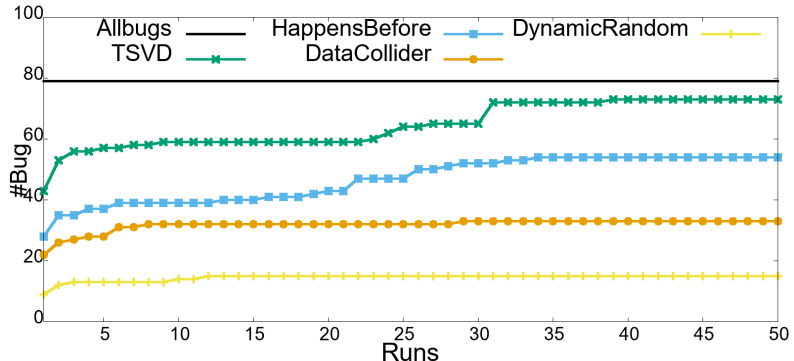
\includegraphics[width=0.8\textwidth]{gfx/TSVDvDataCollider.png}
    \caption{Vergleich TSVD mit Data Collider \cite[173]{li_efficient_2019}}
    \label{fig:TSVDvDataCollider}
\end{figure}
%\end{comment}

In dieser Sektion wird \acs{TSVD} mit Data Collider verglichen. \\
\acs{TSVD} hat in der ersten Runde 42 Bugs und nach zwei Runden 11 weitere Bugs gefunden, während Data Collider signifikant weniger Bugs gefunden hat, was in \ref{fig:TSVDvDataCollider} erkannt werden kann.
\section{Dynamische Race Detection durch Lockset Analyse}

In dieser Sektion wird Dynamische Race Detection durch Lockset Analyse betrachtet und anhand von Eraser nähergebracht. Auf einem hohen Level überprüft Eraser, ob geteilter Speicherzugriff durch einen konsistenten Lock Mechanismus geschützt ist. Auf Locks wird in Kapitel \hyperref[sec:loesen]{5} weiter eingegangen \cite[vgl.][392]{savage_eraser_nodate}.

\subsection*{Eraser}

Erasers Lock Mechanismus ist, ob jeder Zugriff auf eine geteilte Variable durch ein Schloss gesichert ist. Dieser Mechanismus wird überprüft, indem Eraser alle Zugriffe auf den Speicher überwacht. Das Problem dabei ist, dass Eraser nicht weiß, welches Lock für welche Variable ist \cite[vgl.][396]{savage_eraser_nodate}. \\
\\
Um dies herauszufinden, benutzt Eraser Lockset Refinement. Für jede geteilte Variable \texttt{v} hat Eraser ein Set \texttt{C(v)} an möglichen Locks für \texttt{v}. Bei jedem Zugriff auf \texttt{v} von einem Thread wird die Schnittmenge zwischen die aktuellen Locks \texttt{locks\_held} und \texttt{C(v)} gebildet und zurück in \texttt{C(v)} geschrieben. Wenn \texttt{C(v)} nun leer ist liegt ein Data Race vor. Dargestellt ist dieser Mechanismus in \ref{tab:locksetRefinment} \cite[vgl.][396-397]{savage_eraser_nodate}. 

%\begin{comment}
\begin{table}[h]
    \myfloatalign
    \begin{tabularx}{\textwidth}{XXX} \toprule
        \tableheadline{Program} & \tableheadline{locks\_held}
        & \tableheadline{C(v)} \\ 
        \midrule
        lock(mu1); & \{ \} &  \{ mu1, mu2 \} \\
        v := v + 1; & \{ mu1 \} & \{ mu1, mu2 \} \\
        unlock(mu1); & \{ \} & \{ mu1 \} \\
        \midrule
        lock(mu2); & \{ \} & \{ mu1 \} \\
        v := v + 1; & \{ mu2 \} & \{ mu1 \} \\
        unlock(mu1); & \{ \} & \{ \} \\
        \bottomrule
    \end{tabularx}
    \caption[Lockset Refinment]{Lockset Refinment \cite[397]{savage_eraser_nodate}}
    \label{tab:locksetRefinment}
\end{table}
%\end{comment}

\subsubsection*{Verbesserungen von Lockset Refinement}

Der Lock Mechanismus ist jedoch zu restriktiv. Um diesen zu Verbessern nimmt Eraser drei Szenarien aus dem Lock Mechanismus, die ein Data Race verursachen würden, aber keines sind. Diese drei Szenarien sind: Die Initialisierung einer geteilten Variable, Read-Shared Data, also Variablen die nach einmaligen initialisieren nur noch gelesen werden, und Read-Write Locks, welches Variablen sind, auf die nur ein Thread mit Schreiboperationen zugreift \cite[vgl.][396-397]{savage_eraser_nodate}. \\
\\
In \ref{fig:eraserState} dargestellt sind die Zustände, welche eine geteilte Variable bei der verbesserten Version des Lockset Refinements haben kann. Bei der Initialisierung wird der Zustand der Variable auf den \texttt{Virgin} Zustand gesetzt. Sobald ein Thread auf die Variable zugreift, ändert sich der Zustand zu \texttt{Exclusive} und bleibt solange in diesem Zustand bis ein neuer Thread auf die Variable zugreift. Wenn eine Lese Operation von dem neuen Thread ausgeht, ist der neue Zustand \texttt{Shared}. Wird von dem neuen Thread jedoch eine Schreib Operation ausgeführt, geht die Variable in den \texttt{Shared-Modified} Zustand. Um die oben genannten Fälle zu lösen, wird ein Data Race nur im \texttt{Shared-Modified} Zustand berichtet \cite[vgl.][397-399]{savage_eraser_nodate}.   

%\begin{comment}
\begin{figure}[ht]
    \centering
    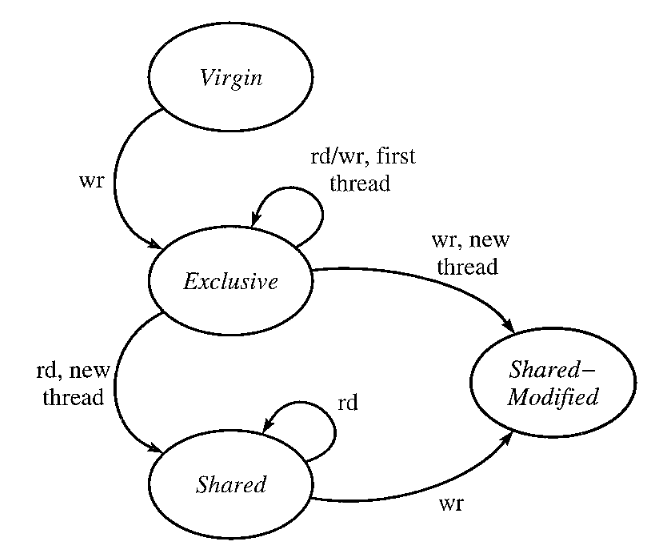
\includegraphics[width=0.5\textwidth]{gfx/eraser_state.png}
    \caption{Eraser States \cite[389]{savage_eraser_nodate}}
    \label{fig:eraserState}
\end{figure}
%\end{comment}

\subsection*{Leistung}

\textcite[vgl.][400]{savage_eraser_nodate} beschreiben, dass Leistung nicht das primäre Ziel bei Eraser war und dementsprechend noch viele Stellen Verbesserungsmöglichkeiten.\\ 
\\
Programme, auf die Eraser angewendet wird, sind um einen Faktor von 10 bis 30 langsamer. Zudem kann Thread Scheduling einen Einfluss auf das Ergebnis von Eraser haben kann \cite[vgl.][400]{savage_eraser_nodate}.   

%\subsection{Auswertung}


\section{Statische Race Detection}

Diese Sektion beschäftigt sich mit Statischer Race Detection. Diese funktioniert in den meisten Algorithmen, wie zum Beispiel Relay \cite[vgl.][208]{relay} oder RacerD \cite[vgl.][57]{nikos_2019}, mittels der Analyse von Locks in einem gegebenen Programm. Diese Analyse ist ähnlich, wie die Dynamische Race Detection durch Lockset Analyse. Die Sektion wird sich auf den von Facebook genutzten RacerD Algorithmus \cite[vgl.][2]{racerd} fokussieren und diesen erklären. 

\subsection*{RacerD}

RacerD analysiert alle nicht private Methoden von Klassen eines gegebenen Programms. Dabei müssen zwei Fragen beantwortet werden, für ein Paar Zugriffe einer Klasse \cite[vgl.][7]{racerd}:

\begin{enumerate}
	\item Sind die Zugriffe auf die selbe Adresse?
	\item Sind die Zugriffe gleichzeitig?
\end{enumerate}
\noindent
Um diese Fragen zu beantworten gibt es in RacerD die Locks, Threads, Ownership und Access Snapshots Domänen \cite[vgl.][7-8]{racerd}. 

\subsubsection*{Locks Domäne}

Die Locks Domäne erkennt, dass kein Data Race entsteht, dadurch, dass das Objekt durch das selbe Lock geschützt wird und deswegen nur ein Thread gleichzeitig drauf zugreifen kann \cite[vgl.][8]{racerd}. RacerD hat als Ziel eine kleine Menge an Data Races zu finden, die mit hohem Vertrauen auch Races sind. Deshalb fokussiert sich RacerD darauf, unsicher Stellen zu finden, die durch kein Lock geschützt sind. Dabei versucht RacerD keine Races zu finden, die entstehen, da das Objekt durch das falsche Lock geschützt sind \cite[vgl.][9]{racerd}. 

\subsubsection*{Threads Domäne}

Die Threads Domäne erkennt, das kein Data Race vorliegt, indem es erfasst, ob eine Stelle nur von einem Thread aufgerufen werden kann \cite[vgl.][8]{racerd}. Um zu festzustellen, ob eine Stelle im Programm mehreren Thread aufgerufen wird $"$concurrent context inferernce$"$ \cite[9]{racerd} genutzt. Dafür gibt es drei abtrakte Zustände.
Gestartet wird im Stadium $"$NoThread$"$. Dieser bedeutet, dass diese Stelle nur auf einem Thread ausgeführt wird \cite[vgl.][9-10]{racerd}.\\
\\
Werden Annotationen, wie \texttt{@ThreadSafe} oder \texttt{@GuardedBy} genutzt, wird in den Zustand $"$AnyThread$"$ übergegangen. In diesem Zustand können Programm Code Stellen, die auf einem Thread laufen, der mit jedem anderen Thread verschachtelt werden kann. Dasselbe gilt auch bei Verwendung des \texttt{synchronized} keyword oder anderen Locks \cite[vgl.][10]{racerd}.\\
\\
Wenn die Annotation \texttt{@UiThread} oder die Methode \texttt{assertMainThread()} benutzt wird ändert sich der Zustand in $"$AnyThreadButMain$"$. Diese Prozeduren laufen auf dem Main Thread und können parallel zu Code in Hintergrund Threads laufen \cite[vgl.][10]{racerd}.

\subsubsection*{Ownership Domäne}

Die Ownership Domäne bezieht sich auf Speicher, welcher nur von einem Thread angesprochen werden kann und dadurch zu keinem Race führen kann. \ref{lst:ownership} gilt als Bespiel hierfür. Die Methode \texttt{ownedAccess()} kann ohne Data Races von mehreren Threads ausgeführt werden. Dies liegt daran, dass die Threads zwar das gleiche ausführen, aber jeder Thread eine neue Instanz \texttt{x} der Klasse \texttt{C} sich erzeugt. Es macht sich die Tatsache zunutze, dass ein neu initialisiertes Objekt über den Befehl \texttt{new} zugewiesen wird \cite[vgl.][10]{racerd}. \\

%\begin{comment}
\begin{lstlisting}[language=Java,frame=tb,caption={Ownership Domäne \cite{racerd}}, label={lst:ownership}, numbers=left, stepnumber=1, captionpos=b, tabsize=4]
void ownedAccess() {
	C x = new C();
	c.x = 42;
}
\end{lstlisting}
%\end{comment}

\subsubsection*{Access Snapshots Domänen}

Die Access Snapshots Domäne nimmt relevante Informationen und speichert sie in einem \texttt{Access Snapshot}, sobald auf Dynamischen Speicher zugegriffen wird \cite[vlg.][11]{racerd}. Gespeichert werden \cite[vgl.][8]{racerd}:
\begin{itemize}
	\item Die Stelle im Speicher, welche aufgerufen wird.
	\item Die Art des Zugriffs, also ob gelesen oder geschrieben wird.
	\item Wie viele Locks gehalten werden.
	\item Ob die Stelle von mehreren Threads ausgeführt wird (Thread Domäne).
	\item Ob die Stelle von nur einem Thread angesprochen werden kann (Ownership Domäne).
\end{itemize}

\subsubsection*{Data Races erkennen}

Um Data Races mit RacerD zu erkennen, wird jedes Paar Access Snapshots miteinander verglichen. Um ein Data Race zu erzeugen müssen beide Access Snapshots auf die selbe Speicherstelle zugreifen und eine Operation auf diese Stelle muss eine Schreiboperation sein. Zudem muss mindestens einer der Zugriffe ohne Lock passieren. Außerdem darf keiner der beiden Access Snapshots nur von einem Thread angesprochen werden. Zuletzt muss der Wert für die Thread Domäne $"$AnyThread$"$ besitzen, also darf mindestens einer der Threads nicht der Main Thread sein \cite[vgl.][8]{racerd}. Wenn ein Race gefunden wurde, wird ein Stacktrace zurückgegeben, sodass man den Bug analysieren kann \cite[vgl.][15]{racerd}.



\chapter{Lösen von Thread Safety Problemen}
 \label{sec:loesen}

Diese Sektion beschäftigt sich damit, wie die zuvor gefundenen Thread Safety Verstöße behoben werden können. Die Erklärung wird Beispielhaft in Java gemacht. Für andere Programmiersprachen gibt es aber ähnliche Methoden, welche man benutzen kann um diese Fehler zu beheben.

\section{Synchronized}

 Java bietet mehrere Optionen zum Lösen der Verstöße. Zum einen bietet Java seit Java 5 die \texttt{java.util.concurrent} Bibliothek, mit der sich der nächste Teil beschäftigt. Zum andern wird das \texttt{synchronized} keyword gestellt, mit dem sich diese Sektion beschäftigt \cite[vgl.][121]{fekete_teaching_nodate}. \\
\\
 Um das \texttt{synchronized} keyword zu erläutern wird das Beispiel, aus den \hyperref[sec:threads]{Theoretische Grundlagen}, \ref{lst:threadSafety}. In \ref{lst:threadSafetySolved} wird eine Klasse beschrieben, die dieselbe Funktionalität wie die Klasse in \ref{lst:threadSafety} hat. Der Unterschied zwischen den Klassen ist, dass \ref{lst:threadSafetySolved} Thread sicher ist und somit von mehreren Threads gleichzeitig aufgerufen werden kann, ohne das Problem entstehen \cite[vgl.][5-6]{brian}. 
\\
%\begin{comment}
 \begin{lstlisting}[language=Java,frame=tb,caption={Thread-safe Sequence Generator \cite{brian}}, label={lst:threadSafetySolved}, numbers=left, stepnumber=1, captionpos=b]
public class Sequenz {
	@GuardedBy("this") private int value;

	public synchronized int getNext() {
		return value++;
	}
}
\end{lstlisting}
%\end{comment}


Das \texttt{synchroized} keyword setzt dabei eine Art Schloss, auch Lock genannt, auf das Objekt, sodass nur ein Thread gleichzeitig darauf zugreifen kann. Wenn also die Methode \texttt{getNext()} von einem Objekt der Klasse \texttt{Sequenz} vom Thread A aufgerufen wird und der Thread B dieselbe Methode des gleichen Objekts aufrufen will, muss Thread B solange warten bis A fertig ist und das Schloss auflöst \cite[vgl.][17]{brian}.



% Optimierung von Synchronization?
 \section{Liveness Hazards}

Ein Problem, dass durch schlechte Synchronisation auftreten kann, sind Liveness Hazards. Diese entstehen, wenn beispielsweise Thread A darauf wartet, dass Thread B eine Ressource, aufhört zu locken, aber Thread B dies nie tut. Diese Art von Liveness Hazard nennt man livelock \cite[vgl.][5-6]{brian}.

%\begin{comment}
\begin{lstlisting}[language=Java,frame=tb,caption={Deadlock \cite{fekete_teaching_nodate}}, label={lst:deadlock}, numbers=left, stepnumber=1, captionpos=b]
class BankAccountA {
    private int balance; 
    private Bank myBank; 

    public synchronized void transfer(BankAccountA target, int amount) throws DifferentBankException {
        if (myBank != target.myBank) 
            throw new DifferentBankException(); 
        
        balance -= amount; 
        synchronized(target) { 
            target.balance += amount; 
        } 
    }
}
\end{lstlisting}
%\end{comment}

Ein weiterer Liveness Hazard ist der Deadlock \cite[vgl.][6]{brian}. Dieser entsteht, wenn verschiedene Threads sich gegenseitig blockieren und dadurch kein Thread weitere Aufgabe ausführen kann. Ein Beispiel hierfür ist \ref{lst:deadlock}. Problem hierbei ist, dass wenn das \texttt{target} gleich dem auszuführenden BankAccountA ist, das \texttt{target} nicht gelocked werden kann in Zeile 10, da es bereits durch den Funktionsaufruf gelocked ist \cite[vgl.][122]{fekete_teaching_nodate}. 
\\
%\begin{comment}
\begin{lstlisting}[language=Java,frame=tb,caption={Deadlock Lösung \cite{fekete_teaching_nodate}}, label={lst:deadlockLösung}, numbers=left, stepnumber=1, captionpos=b]
class BankAccountB { 
    private int balance; 
    
    private Bank myBank; 

    public void transfer(BankAccountB target, int amount) throws DifferentBankException { 
        if (myBank != target.myBank)
            throw new DifferentBankException(); 
        
        synchronized(myBank) { 
            balance -= amount; 
            target.balance += amount; 
        } 
    }
}
\end{lstlisting}
%\end{comment}

In \ref{lst:deadlockLösung} ist dieselbe Funktion dargestellt, mit dem Unterschied, dass diese keinen Deadlock erzeugt. Der Unterschied in der Klasse \texttt{BackAccountB} ist, dass am Anfang der Funktion nicht das Objekt gelocked wird und dadurch das vorher beschriebene Problem nicht mehr auftreten kann \cite[vgl.][122]{fekete_teaching_nodate}.

 \chapter{Zusammenfassung}
 \section{Fazit}

Ziel der Arbeit war es, den Lesenden zu zeigen, was Thread Safety ist und warum man es braucht. Des Weiteren sollte die Arbeit erläutern, wie man Verstöße erkennt und erkannte Verstöße löst.

Was Thread Safety ist und wie ein Data Race entsteht, wurde in den \hyperref[sec:threadSafety]{Theoretischen Grundlagen} erklärt.


Anschließend wurde darauf eingegangen, wie man durch Dynamische bzw. Statische Race Detection Data Races in einem Programm erkennen kann. Dabei wurde die Dynamische Race Detection zwischen der \acs{HB} Beziehung und dem Lockset Algorithmus unterschieden.

Zuletzt wurde beispielhaft an dem Synchronized Keyword in Java erklärt, wie man die gefunden Data Races beheben kann und welche Probleme, also Deadlocks oder Livelocks, entstehen können, wenn man schlechte Synchronization verwendet. 
 \section{Ausblick}

In der Zukunft könnte man weitere Vergleiche zwischen Statischer und Dynamischer Race Detection erstellen. Zudem kann man weitere Algorithmen zur Statischen, beziehungsweise Dynamischen Data Race Detection betrachten, die eine höhere Anzahl an Bugs finden und schneller bei dem Suchprozess agieren.

%*************************************************************************
% Backmatter
%*************************************************************************
\appendix
%\renewcommand{\thechapter}{\alph{chapter}}
\cleardoublepage
%\part{Appendix}
%\include{chapters/examples/appendix01}
%\include{chapters/examples/appendix02}
%*************************************************************************
% Other Stuff in the Back
%*************************************************************************
\cleardoublepage%********************************************************************
% Bibliography
%*******************************************************
% work-around to have small caps also here in the headline
% https://tex.stackexchange.com/questions/188126/wrong-header-in-bibliography-classicthesis
% Thanks to Enrico Gregorio
\defbibheading{bibintoc}[\bibname]{%
  \phantomsection
  \manualmark
  \markboth{\spacedlowsmallcaps{#1}}{\spacedlowsmallcaps{#1}}%
  \addtocontents{toc}{\protect\vspace{\beforebibskip}}%
  \addcontentsline{toc}{chapter}{\tocEntry{#1}}%
  \chapter*{#1}%
}
\printbibliography[heading=bibintoc]

%*************************************************************************
% Game Over: Restore, Restart, or Quit? Quit
%*************************************************************************
\end{document}
%*************************************************************************
